\documentclass[11pt,letterpaper]{article}
\PassOptionsToPackage{hyphens}{url}
\usepackage[margin=.83in,top=.8in,bottom=.8in,headheight=15pt]{geometry}
\usepackage[T1]{fontenc}
\usepackage{lmodern,amsmath,amssymb,mathtools,bm,booktabs,array,graphicx,tikz}
\usetikzlibrary{arrows.meta,positioning,calc,decorations.pathreplacing,patterns}
\definecolor{ink}{HTML}{17344D}\definecolor{accent}{HTML}{087E8B}\definecolor{pale}{HTML}{EDF5F5}\definecolor{gold}{HTML}{AD6B19}
\providecommand{\dd}{\,\mathrm{d}}\providecommand{\R}{\mathbb{R}}
\providecommand{\E}{\mathbb{E}}\providecommand{\Var}{\operatorname{Var}}
\providecommand{\Cov}{\operatorname{Cov}}\providecommand{\diag}{\operatorname{diag}}
\providecommand{\norm}[1]{\left\lVert#1\right\rVert}
\providecommand{\abs}[1]{\left|#1\right|}
\usepackage{microtype,hyperref,fancyhdr,enumitem,amsthm,sectsty,needspace}
\allsectionsfont{\raggedright}
\hypersetup{colorlinks=true,linkcolor=ink,urlcolor=accent,pdfauthor={Zan Ahmad},pdftitle={Image coordinates, pixel-cell meshes and geometric sensitivity / Lecture notes}}
\setlength{\parindent}{0pt}\setlength{\parskip}{6pt}\linespread{1.07}
\setlist{itemsep=3pt,topsep=4pt,leftmargin=*}
\emergencystretch=2em\clubpenalty=10000\widowpenalty=10000
\pagestyle{fancy}\fancyhf{}\fancyhead[L]{\small Computational Cardiology}\fancyhead[R]{\small Lecture 11}
\fancyfoot[L]{\footnotesize Zan Ahmad}\fancyfoot[R]{\footnotesize\thepage}\renewcommand{\headrulewidth}{.3pt}
\newtheorem{proposition}{Proposition}\newtheorem{theorem}{Theorem}\newtheorem{lemma}{Lemma}
\theoremstyle{definition}\newtheorem{definition}{Definition}\newtheorem{example}{Example}
\numberwithin{equation}{section}
\begin{document}
{\small\scshape Computational Cardiology\hfill Lecture 11}\par\medskip
{\raggedright\hyphenpenalty=10000\exhyphenpenalty=10000\LARGE\bfseries\color{ink} Image coordinates, pixel-cell meshes and geometric sensitivity\par}\medskip
{\small Lecture notes}\par\bigskip
A medical image supplies an array together with a spatial coordinate system. Thresholding, coordinate transformation and mesh construction are separate operations. Their effects can be derived explicitly for a two-dimensional pixel-cell mesh, allowing geometric scale and segmentation decisions to be distinguished.

\section{Intensity arrays and spatial metadata}
\hypertarget{note-intensity-arrays-and-spatial-metadata}{}\label{note:intensity-arrays-and-spatial-metadata}
{\small \href{slides.html\#frame=an-intensity-array-and-a-geometric-image\&step=1}{Slides for this section}}\par
An image-based model begins with a chain of decisions. Our question is whether a change in a reported chamber area comes from the segmentation, the physical scale, or the mesh construction. Those are different causes, so we keep separate objects for intensity values, the binary mask, spatial metadata and mesh connectivity. The companion makes every object from a synthetic generator; the ellipse-like foreground is an instructional shape, not an anatomical reconstruction. That controlled origin gives us a reference mask without pretending that expert clinical annotation is perfect.

The stored image has 28 rows and 36 columns. Its values lie between zero and one and represent arbitrary synthetic intensity. They are not millimeters, pressure or a probability of disease. The generator combines overlapping ellipses, blurs the ideal mask, and adds a small reproducible noise field. Blurring means that a sharp reference boundary becomes a band of intermediate intensities. A threshold converts that band into a discrete choice. The choice should be recorded even if the resulting outline looks convincing.

The pipeline figure deliberately shows indices on the left and physical coordinates on the right. A screenshot alone cannot establish that two images occupy the same place. SimpleITK's Images section identifies size, spacing, origin and direction as the spatial description; it also emphasizes consistent units. In this lesson we adopt millimeters explicitly. We retain the array and metadata together rather than infer physical scale from display width.

The intensity function $I_{r,c}$ and the physical point $x_{r,c}$ are distinct objects. A threshold $t$ defines a mask $M_t=\{(r,c):I_{r,c}\ge t\}$, but it supplies no length scale. Area becomes meaningful only after a spatial map and physical unit are attached.
\section{The affine index-to-physical map}
\hypertarget{note-the-affine-index-to-physical-map}{}\label{note:the-affine-index-to-physical-map}
{\small \href{slides.html\#frame=the-physical-coordinate-map\&step=1}{Slides for this section}}\par
NumPy indexing uses row first and column second. Our geometric point vector instead lists column then row, corresponding to local x then local y. Let the column spacing be 1.25 mm and row spacing be 2 mm. Multiply these spacings by the respective indices, rotate the resulting local displacement, then add the physical origin. Matrix multiplication order matters: rotating an index vector and then applying unequal spacings generally produces a different answer. The direction matrix in this companion is a proper rotation; it preserves lengths and signed area after spacing has been applied.

The origin is the center of pixel zero, not its lower-left corner. A pixel cell extends half a spacing on either side of its center. Therefore the lower-left corner of pixel at column c, row r uses indices c minus one half and r minus one half. Confusing center and corner conventions translates the boundary. Translation leaves area unchanged, so an area check alone cannot catch that error. We additionally test the location of index zero and inspect coordinate orientation.

For our rotation of 20 degrees, positive columns and positive rows point along rotated axes. The implementation rejects nonpositive spacing and unsupported direction matrices instead of silently producing an ambiguous mesh. This is a deliberate scope restriction of the teaching implementation, not a claim that all imaging formats use this particular orientation convention.

\[
\mathbf{x}=\mathbf{o}+D\,\mathrm{diag}(s_x,s_y)\begin{bmatrix}c\\r\end{bmatrix}
\]
Origin and position are in mm; spacings are mm per index increment; D is a dimensionless proper rotation.

Let $A=D\operatorname{diag}(s_x,s_y)$. Translation changes locations but not edge differences. The signed area scale is
\[
 \det A=\det D\,s_xs_y=s_xs_y
\]
for the proper rotations accepted here. Applying unequal spacing after rotation would use a different matrix, since in general $D\operatorname{diag}(s_x,s_y)\ne\operatorname{diag}(s_x,s_y)D$.

\paragraph{Calculation.} With no rotation, origin (\ensuremath{-}20,\ensuremath{-}10) mm, spacing (1.25,2) mm, locate row 3, column 4.

Write the geometric index vector as (4,3), not (3,4).

The displacement is (1.25\ensuremath{\times}4, 2\ensuremath{\times}3) = (5,6) mm.

Add the origin: (\ensuremath{-}20,\ensuremath{-}10)+(5,6) = (\ensuremath{-}15,\ensuremath{-}4) mm.

The point is (\ensuremath{-}15,\ensuremath{-}4) mm. An index-order swap would produce (\ensuremath{-}16.25,\ensuremath{-}2) mm.
\section{Oriented triangles and mask area}
\hypertarget{note-oriented-triangles-and-mask-area}{}\label{note:oriented-triangles-and-mask-area}
{\small \href{slides.html\#frame=triangulating-the-selected-cells-panel-1\&step=1}{Slides for this section}}\par
Thresholding at 0.5 selects 295 pixels in the default image. Each foreground pixel becomes a physical rectangle, split along a consistent diagonal into two triangles. Adjacent cells share the same vertex indices. This produces a conforming mesh of the pixel-cell union, rather than a set of disconnected triangles that merely overlap in a plot. The companion removes unused grid vertices and saves coordinates and connectivity in geometry-data.npz. There are 590 triangles and 337 used vertices in the default construction.

The signed determinant formula gives each triangle's area. Positive signs check the chosen counterclockwise ordering, while the sum checks agreement with the pixel-cell area. Every triangle has area 1.25 square millimeters within floating-point tolerance. Shared edges occur twice and boundary edges once. These checks would reveal reversed ordering or duplicate elements, but they do not prove that a mesh is suitable for a fluid solver. A three-dimensional simulation would additionally need a valid volume mesh, appropriately labeled boundaries, physical models and solver verification.

An exact area match here means the representation of this particular mask is consistent. It does not establish that the mask is anatomically correct. Our staircase boundary remains a consequence of pixel resolution. Smoothing it would be a new geometry operation whose effect on area, connectivity and narrow features must be measured separately.

\[
A_T=\tfrac12\det\!\begin{bmatrix}x_2-x_1&x_3-x_1\\y_2-y_1&y_3-y_1\end{bmatrix},\qquad A_M=N_f s_xs_y
\]
Triangle vertex coordinates are in mm; both areas are in mm\ensuremath{^{2}}; N\_f is the foreground pixel count.

Each foreground pixel has four corner coordinates obtained from $(c\pm\tfrac12,r\pm\tfrac12)$. A consistent diagonal divides its area $s_xs_y$ into two triangles of area $s_xs_y/2$. Adjacent pixels share indexed vertices and edges, so the mesh represents the union of selected cells without internal overlaps.
\begin{center}\begin{minipage}{.98\linewidth}\centering
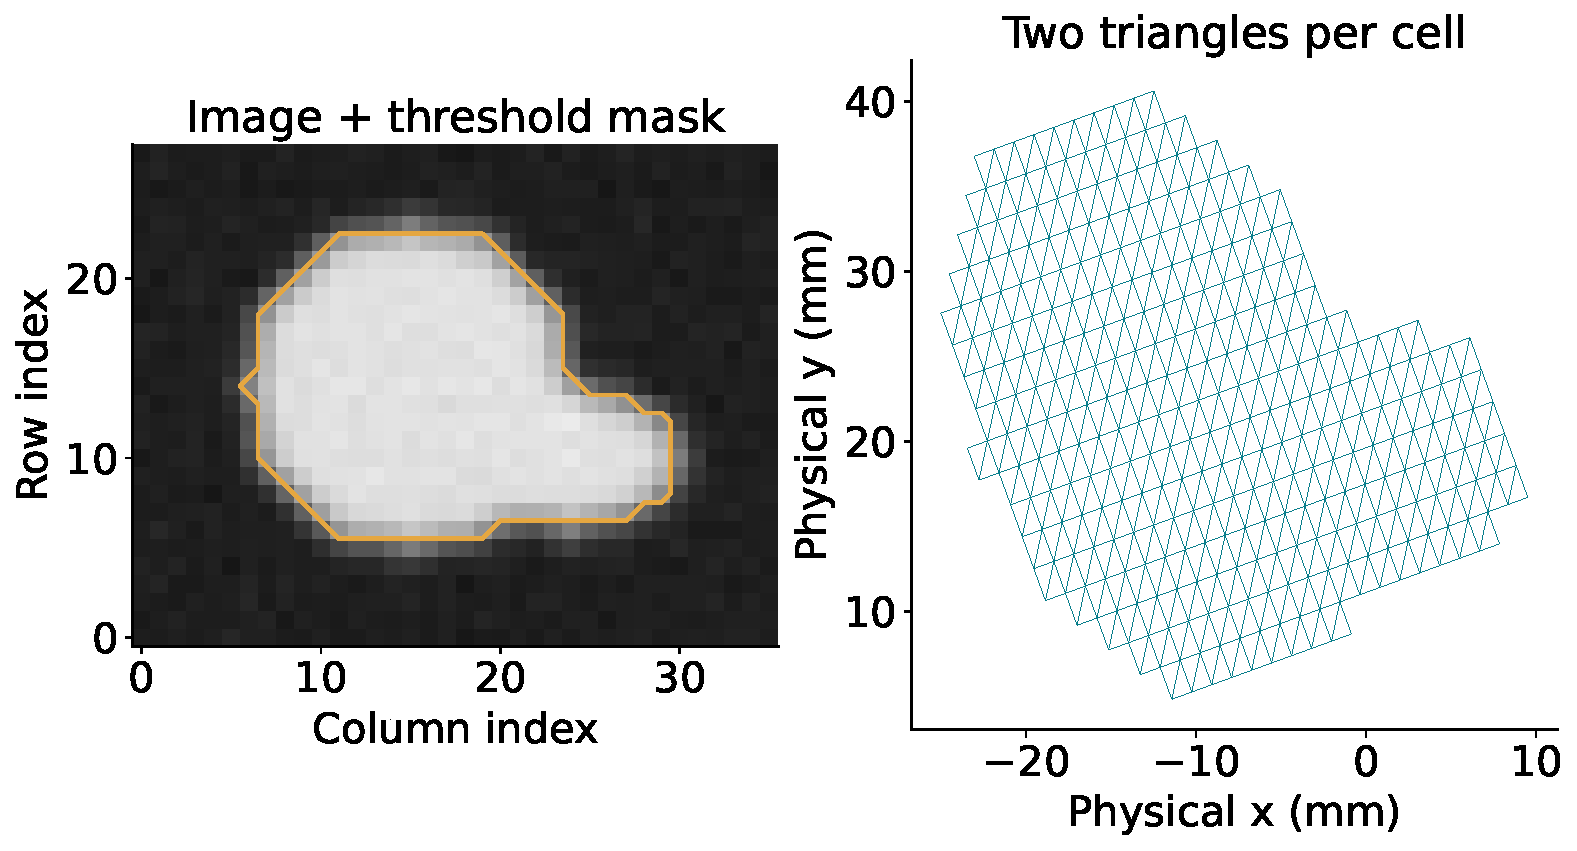
\includegraphics[width=.96\linewidth,height=.57\textheight,keepaspectratio]{image-mesh.pdf}\par\smallskip
{\small Original synthetic image and actual 2D mesh. The 0.5 mask has 295 cells and 590 triangles; area is 737.5 mm$^2$. Index axes and physical axes are intentionally different.}
\end{minipage}\end{center}
\section{Threshold sets and geometric summaries}
\hypertarget{note-threshold-sets-and-geometric-summaries}{}\label{note:threshold-sets-and-geometric-summaries}
{\small \href{slides.html\#frame=threshold-sets-are-nested-panel-1\&step=1}{Slides for this section}}\par
The threshold sweep changes one decision while holding the image and spatial metadata fixed. Higher thresholds cannot add foreground under the greater-than-or-equal rule, so the masks must be nested. The default sweep from 0.35 to 0.65 decreases area from 815 to 682.5 square millimeters. All seven masks remain one component with four-neighbor connectivity. That last fact is a result for this image, not a guarantee that other images preserve a narrow connection.

We also report the diameter of a circle with the same area. This is a scalar summary, not a fitted circle or the width of an appendage. Because diameter depends on the square root of area, its relative changes are smaller. A threshold sensitivity range is not a confidence interval: no probability distribution over plausible thresholds has been supplied. A defensible report names the perturbed parameter, the chosen range and what stayed fixed.

Refining triangles inside an unchanged pixel cell cannot improve the underlying image boundary. Likewise, doubling both physical spacings quadruples every area even though the mask is identical. These controls distinguish implementation consistency, segmentation sensitivity and physical-scale uncertainty. They should be examined before interpreting a downstream flow change.

\[
d_{\mathrm{eq}}=2\sqrt{A_M/\pi}
\]
Area is in mm\ensuremath{^{2}} and equivalent diameter is in mm. This defines a geometric summary, not a flow law.

For $t_2>t_1$, the threshold sets satisfy $M_{t_2}\subseteq M_{t_1}$, hence $A(t_2)\le A(t_1)$. No such monotonicity follows for the number of connected components: removing foreground can split a bridge or remove an isolated component. The equivalent diameter has differential
\[
 d_{eq}=2\sqrt{A/\pi},\qquad\frac{\delta d_{eq}}{d_{eq}}=\frac12\frac{\delta A}{A}.
\]
It summarizes area rather than maximum width or anatomical shape.
\begin{center}\begin{minipage}{.98\linewidth}\centering
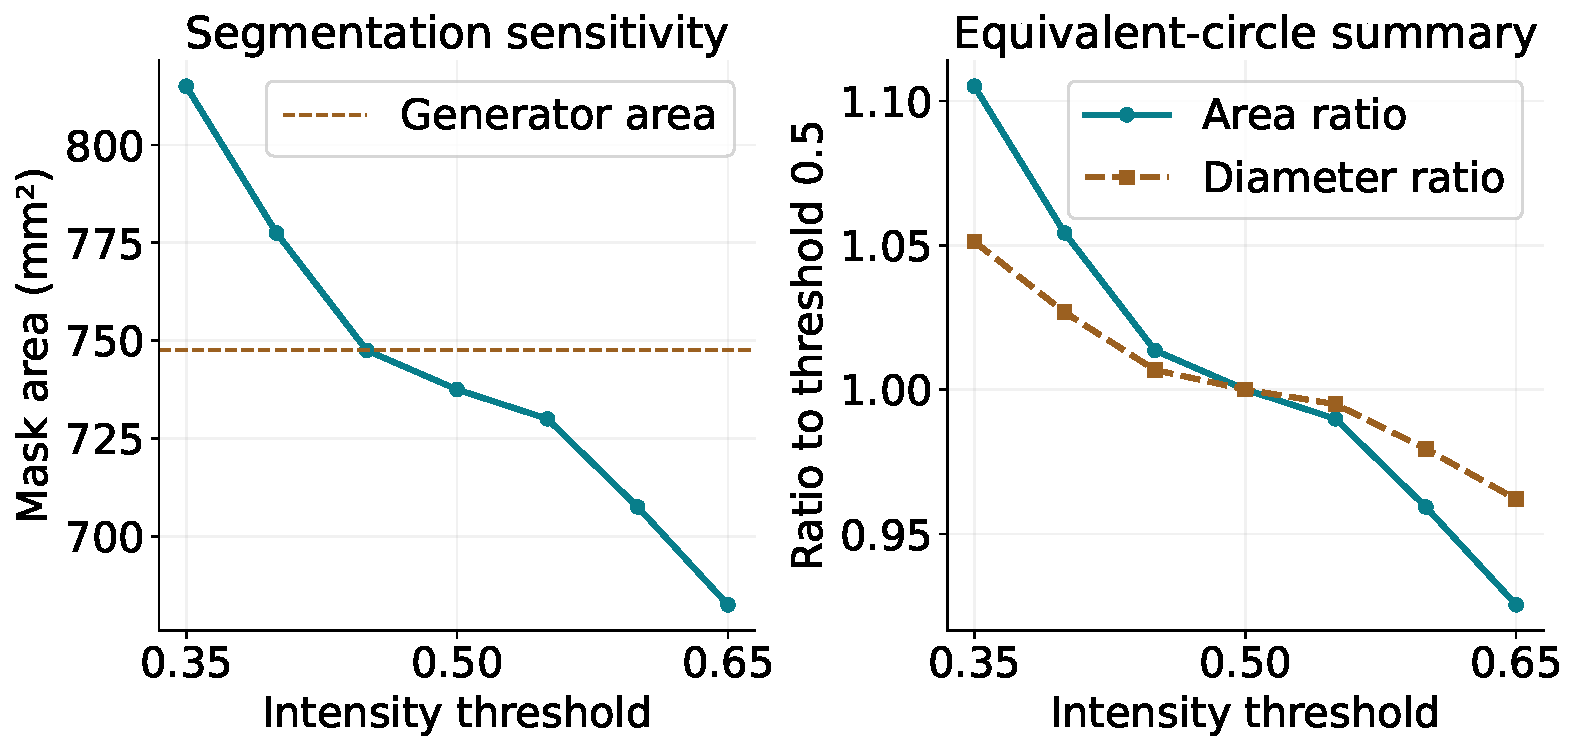
\includegraphics[width=.96\linewidth,height=.57\textheight,keepaspectratio]{geometry-sensitivity.pdf}\par\smallskip
{\small Same input and metadata, seven thresholds. The reference line is the generator mask area, 747.5 mm$^2$. Equivalent diameter refers to an equal-area circle; ratios use threshold 0.5 as their denominator.}
\end{minipage}\end{center}
\section{Resampling and geometric provenance}
\hypertarget{note-resampling-and-geometric-provenance}{}\label{note:resampling-and-geometric-provenance}
{\small \href{slides.html\#frame=label-resampling\&step=1}{Slides for this section}}\par
The provenance file records the generator seed, intensity-array hash and byte convention, shape, threshold comparison, spatial metadata, unit, library versions and mesh construction rule. A hash can establish byte identity under a stated encoding; it cannot establish correct units or biological validity. Two analysts can hash identical arrays yet disagree geometrically if one discards spacing. Conversely, tiny differences in a regenerated noise field can change a few boundary pixels, so store the actual synthetic array as well as the seed.

When resampling labels, the SimpleITK Resampling section describes nearest-neighbor interpolation as preserving the label set. That does not promise preservation of a thin feature or its area. Record the target grid and transform direction, then recheck geometry. Keep interpolation of intensities distinct from interpolation of class labels. The present construction performs no resampling, so threshold sensitivity is isolated from interpolation effects.

Changing both spacings by a factor $a$ changes area by $a^2$ and equivalent diameter by $a$, while leaving pixel counts unchanged. A coordinate-origin error can leave all these scalar quantities unchanged. Therefore area consistency cannot determine whether a mesh is correctly located or oriented.
\section{Representation error and physical interpretation}
\hypertarget{note-representation-error-and-physical-interpretation}{}\label{note:representation-error-and-physical-interpretation}
{\small \href{slides.html\#frame=scale-and-location-have-different-signatures\&step=1}{Slides for this section}}\par


Refining a triangle inside a selected pixel changes the mesh resolution but not the pixel-cell union. It cannot recover an unresolved anatomical boundary. Conversely, a change to the mask boundary changes the represented domain even if the subsequent triangulation is exact. The synthetic construction establishes internal geometric consistency; anatomical validity requires an independent image interpretation.
\bigskip
\section*{Exercises}
\par\noindent\begin{minipage}{\linewidth}
\subsection*{AC11-E1. Audit a spatial map}
Use origin (10,-5) mm, spacing (2,3) mm and a 90-degree counterclockwise rotation D =\allowbreak{} [[0,-1],[1,0]].

\textbf{a} Locate the center at row 2, column 4.

\end{minipage}\par\medskip
\textbf{b} Locate the lower-left cell corner in local index coordinates and map it physically.

\textbf{c} What is the cell area, and does changing only the origin alter it?

\par\noindent\begin{minipage}{\linewidth}
\subsection*{AC11-E2. Check triangle orientation}
A triangle has vertices A=\allowbreak{}(0,0), B=\allowbreak{}(2,0), C=\allowbreak{}(2,3), all in millimeters.

\textbf{a} Compute signed area in order A,B,C.

\end{minipage}\par\medskip
\textbf{b} Compute signed area after swapping B and C. What should the mesh check report?

\textbf{c} Two triangles form the 2 mm by 3 mm rectangle. Explain why an area sum of 6 mm$^2$ is necessary but insufficient for solver readiness.

\par\noindent\begin{minipage}{\linewidth}
\subsection*{AC11-E3. Separate segmentation and scale}
A mask changes from 400 to 361 pixels when its threshold rises. Spacing remains (0.5,0.8) mm.

\textbf{a} Find both areas and the signed percent area change.

\end{minipage}\par\medskip
\textbf{b} Find the ratio of equivalent-circle diameters without calculating pi.

\textbf{c} If both spacings are accidentally doubled, how do area and equivalent diameter change for either fixed mask?

\par\noindent\begin{minipage}{\linewidth}
\subsection*{AC11-E4. Write a reproducibility receipt}
A colleague sends only mask.png and says it is ready for cardiac CFD.

\textbf{a} Name four missing items needed to reproduce its physical geometry.

\end{minipage}\par\medskip
\textbf{b} Give one implementation check and one independent validation question.

\textbf{c} State three additional ingredients a 3D flow calculation needs beyond this lesson's 2D mesh.

\section*{References}
\noindent\begin{minipage}{\linewidth}
Zan Ahmad, Advanced Topics in Computational Cardiology syllabus, Fall 2024. PDF pages 1--2.

\end{minipage}\par\medskip
\noindent\begin{minipage}{\linewidth}
SimpleITK, Fundamental Concepts. Images; Resampling; Resampling---Common Errors.

\url{https://simpleitk.readthedocs.io/en/master/fundamentalConcepts.html}
\end{minipage}\par\medskip
\end{document}
